\documentclass[punct]{ctexbeamer}
%\documentclass{beamer}
\usefonttheme{professionalfonts}   % 数学公式字体
%\usepackage{ctex}
%
%%\usepackage{tabularx} % for 'tabularx' env. and 'X' col. type
%\usepackage{ragged2e} % for \RaggedRight macro
%\usepackage{booktabs} % for \toprule, \midrule etc macros
%%% create a derivative column type called 'L':
%\newcolumntype{L}{>{\RaggedRight\hangafter=1\hangindent=0em}X}

%\usepackage{mma}
\usepackage{colortbl}  %彩色表格需要加载的宏包
\usepackage{xcolor}
\titlegraphic{
\includegraphics[width=2cm]{tjnu.jpg}}

\usepackage{color}
%\lineskip=9pt
\linespread{1.2}\selectfont
\makeatletter
\renewcommand\normalsize{%
	\@setfontsize\normalsize\@xpt\@xiipt
	\abovedisplayskip 3\p@ \@plus3\p@ \@minus3\p@
	\abovedisplayshortskip \z@ \@plus3\p@
	\belowdisplayshortskip 3\p@ \@plus3\p@ \@minus1\p@
	\belowdisplayskip \abovedisplayskip
	\let\@listi\@listI}
\makeatother
\parskip=6pt


\usetheme{Madrid}
\useinnertheme{circles}
\setbeamertemplate{navigation symbols}{}
%\setbeamertemplate{footline}[page number]
\setbeamertemplate{footline}[frame number]{}
\usepackage{lmodern}
\usepackage{amsmath}
\usepackage{amssymb}
\usepackage{latexsym}
\usepackage{amsthm}
\usepackage{mathrsfs}
\usepackage{mathrsfs}
\usepackage{graphicx}
\usepackage{subcaption}
\usepackage{mma}

\setbeamertemplate{theorems}[numbered]
\newtheorem{thm}{定理}[section]
\newtheorem{prop}[thm]{命题}
\newtheorem{cor}[thm]{推论}
\newtheorem{defi}[thm]{定义}
\newtheorem{lem}[thm]{引理}
\newtheorem{iden}{恒等式}
\newtheorem{identity}{等式}
\newtheorem{coro}{推论}

\newtheorem{quest}[thm]{问题}
\newtheorem{xiti}[thm]{习题}
\newtheorem{conj}[thm]{猜想}
\newtheorem{ex}{例}[section]

\definecolor{blue}{rgb}{0,0.08,1}
\newcommand{\blue}{\textcolor{blue}}
\def\pf{\noindent {\bf 证明\ }}

\begin{document}

\title{组\ 合\ 数\ 学}

\author{张\ 彪}
\institute[数学科学学院]{\normalsize 天津师范大学}
%\date[2011年10月13日]{\small 2011年10月13日}
\date[]{zhang@tjnu.edu.cn}

\frame[plain]{\titlepage}


\begin{frame}
    %    {二项式系数}

    二项式定理中的系数 都是组合数,组合数和二项式定理有密切的关系.

    本章我们就详细讨论这种关系.


    回忆:  表达式$\binom{n}{k}$表示 $n$元集合的$k$元子集的个数.




    %由于它们出现在二项式定理中,因此也叫做二项式系数.

    对于非负整数$n$和$k$, 我们已经证明了\vspace{8pt}
    $$
    \binom{n}{k}=\left\{\begin{array}{cc}
        \frac{n!}{k!(n-k)!} &1 \le {k} \le {n}
        \\[6pt]
        {0} & {k}>n
        %        \\[6pt]
        %        {0} & {k} < 0
    \end{array}\right.$$

    由此 不难得到


    \begin{itemize}

        \item 对称性:  $\binom{n}{k}=\binom{n}{n-k}$

        \item 恒等式: $\binom{n}{0}+\binom{n}{1}+\cdots+\binom{n}{n}=2^{n}$


    \end{itemize}


    它还具有许多很奇妙的性质,关于它也有着许多恒等式.
    %当$k>n$时,  ${n \choose k}=0.$

    %当$0 \le k \le n$时,
    %\[\binom{n}{k}=\frac{n!}{k!(n-k)!}\]

    %特别地,
    %$${n \choose 0}={n \choose n}=1$$
\end{frame}


\begin{frame}{第$3$章\quad 二项式系数}
\tableofcontents
\end{frame}
\AtBeginSection[]
{
	\begin{frame}
	\frametitle{二项式系数}
	\tableofcontents[currentsection]
\end{frame}
}
\section{Pascal公式}

\begin{frame}
%    {Pascal公式}



Pascal公式给出了二项式系数的\blue{递推关系}.
\begin{thm}[Pascal公式]

对于满足$1\leq k\leq n-1$的所有整数$k$和$n$,
\[
	\binom{n}{k}=\binom{n-1}{k}+\binom{n-1}{k-1}.
	\]
\end{thm}
%
%\blue{边值条件}
%${n \choose 0}={n \choose n}=1$
%


利用\blue{边值条件}
${n \choose 0}={n \choose n}=1$  和 Pascal公式 可以得到下面的表格:
\begin{table}[]
    \begin{tabular}{c|cccccc}
        $n\backslash k$ & 0 & 1 & 2  & 3  & 4 & 5 \\ \hline
        0 & 1 &   &    &    &   &   \\
        1 & 1 & 1 &    &    &   &   \\
        2 & 1 & 2 & 1  &    &   &   \\
        3 & 1 & 3 & 3  & 1  &   &   \\
        4 & 1 & 4 & 6  & 4  & 1 &   \\
        5 & 1 & 5 & 10 & 10 & 5 & 1 \\
    \end{tabular}
\caption{Pascal三角}
\end{table}

\vspace{-10pt}


\pause
证明:直接将$\binom{n}{k}=\frac{n!}{k!\cdot(n-k)!}$代入上式验证等式成立.
\end{frame}



\begin{frame}{Pascal三角  (杨辉三角 或 贾宪三角)}
\begin{center}
\begin{minipage}{0.5\linewidth}
    17世纪, 法国数学家Pascal做出了下面的三角形.
    %        ,西方通常叫做Pascal三角.
    \begin{table}[]
        \begin{center}
            1

            1 \quad 1

            1\quad	\quad2\quad	\quad1

            1\quad	\quad  3\quad\quad3\quad\quad	1

            1\quad	\quad 4 \quad\quad	6\quad\quad	4\quad \quad	1

            1\quad\quad	5\quad\quad	10\quad\quad	10\quad\quad	5\quad\quad	1

            1\quad\quad	6\quad\quad	15\quad\quad	20\quad\quad	15\quad\quad	6\quad\quad	1

        \end{center}
        \caption{Pascal三角}
        %    \caption{杨辉三角 或 贾宪三角}
    \end{table}
\end{minipage}
\hspace*{25pt}
\begin{minipage}{0.35\linewidth}
    \begin{figure}
        \centering
        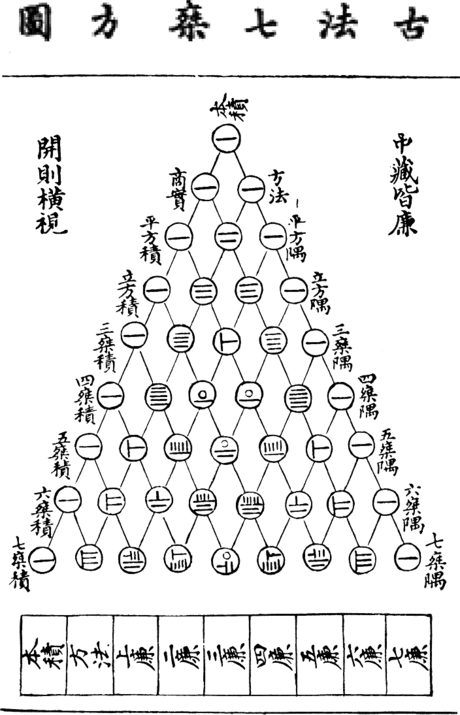
\includegraphics[scale=0.21]{yanghui.png}
        \caption{朱世杰《四元玉鉴》中的“古法七乘方图''}
    \end{figure}
\end{minipage}
\end{center}






    13世纪中国南宋数学家杨辉在《详解九章算术》里解释右边这种形式的数表,并说明此表引自11世纪贾宪的《释锁算术》.

    %贾宪还对贾宪三角表(古代称数字表为“立成”)的构造进行描述.
    %贾宪的三角表图和文字描写,仍保存在大英博物馆所藏《永乐大典》卷一万六千三百四十四.


    %在我国称这个三角形为杨辉三角形, 1250年由杨辉提出.
\end{frame}



%\begin{frame}{$\binom{n}{k}=\binom{n-1}{k}+\binom{n-1}{k-1}$的组合证明}
%
%
%\begin{minipage}{0.48\linewidth}
%	\begin{itemize}
%	\item 令$S$是$n$元集合,
%    考虑它的$k$元子集
%
%    \item 任取$x \in S$,将$S$的$k$元子集按$x$分成两大类:
%        \begin{center}
%        $A$ \, =\, \{不含元$x$的$k$元子集\} \\
%        $B$ \, =\, \{包含元$x$的$k$元子集\}
%        \end{center}
%    \item  按加法原理,$\binom{n}{k}=|A|+|B|$
%
%	\item $A$的$k$元子集恰好是集合$S-\{x\}$的$k$元子集,故$$|A|=\binom{n-1}{k}$$
%
%
%\item  $B$的$k$元子集是通过将$x$添加到集合$S-\{x\}$的($k-1$)元子集得到的,故$$|B|=\binom{n-1}{k-1}.$$
%	\end{itemize}
%\end{minipage}
%\begin{minipage}{0.5\linewidth}
%\begin{flushleft}
%\quad 例如:
%
%\begin{itemize}
%\item $S=\{x,a,b,c,d\}$,
%
%$n=5$,$k=3$,$\binom{n}{k}=10$
%
%
%\item $A$的3元子集:
%
%\begin{center}
%$\{a,b,c\}$, $\{a,b,d\}$,
%
%$\{a,c,d\}$, $\{b,c,d\}$,
%\end{center}
%
%对应集合$\{a,b,c,d\}$的3元子集
%
%
%\item  $B$的3元子集:
%
%\begin{center}
%$\{x,a,b\}$, $\{x,a,c\}$, $\{x,a,d\},$
%
%$\{x,b,c\}$, $\{x,b,d\}$, $\{x,c,d\}$,
%\end{center}
%
%
%去掉$x$后,得
%
%\begin{center}
%$\{a,b\}$, $\{a,c\}$, $\{a,d\}$,
%
%$\{b,c\}$, $\{b,d\}$, $\{c,d\}$,
%\end{center}
%
%恰好是集合$\{a,b,c,d\}$的2元子集.
%\end{itemize}
%
%\end{flushleft}
%\end{minipage}
%
%
%\end{frame}

\begin{frame}{$\binom{n}{k}=\binom{n-1}{k}+\binom{n-1}{k-1}$的组合证明 --- 集合的组合}


    \begin{minipage}{0.49\linewidth}
        \begin{itemize}
            \item 令$S=\{1,2,\cdots,n\}$,\\
            考虑它的$k$元子集的个数

            \item 将$S$的$k$元子集分成两类:
            \begin{center}
                $A$ \, =\, \{不含元$n$的$k$元子集\} \\
                $B$ \, =\, \{包含元$n$的$k$元子集\}
            \end{center}
            \item  按加法原理,$\binom{n}{k}=|A|+|B|$.

            \item $A$中的$k$元子集恰好是集合 $\{1,2,\cdots,n-1\}$的$k$元子集,故$|A|=\binom{n-1}{k}$


            \item  $B$的$k$元子集已包含$n$,只需从集合$\{1,2,\cdots,n-1\}$中再选出 $k-1$个元素即可,故$|B|=\binom{n-1}{k-1}.$
        \end{itemize}
    \end{minipage}
    \begin{minipage}{0.49\linewidth}
        \begin{flushleft}
            \quad 例如:

            \begin{itemize}
                \item  $n=5$, $k=3$, $\binom{n}{k}=10$

                $S=\{1,2,3,4,5\}$,




                \item

                \small{$A$的3元子集

                    \begin{center}
                        $\{1,2,3\}$, $\{1,2,4\}$,

                        $\{1,3,4\}$, $\{2,3,4\}$,
                    \end{center}

                    对应集合$\{1,2,3,4\}$的3元子集.}


                \item  \small{$B$的3元子集

                    \begin{center}
                        $\{1,2,5\}$, $\{1,3,5\}$, $\{1,4,5\},$

                        $\{2,3,5\}$, $\{2,4,5\}$, $\{3,4,5\}$,
                    \end{center}


                    去掉元素$n=5$后,得

                    \begin{center}
                        $\{1,2\}$, $\{1,3\}$, $\{1,4\}$,

                        $\{2,3\}$, $\{2,4\}$, $\{3,4\}$,
                    \end{center}

                    恰好是集合$\{1,2,3,4\}$的2元子集.}
            \end{itemize}

        \end{flushleft}
    \end{minipage}


\end{frame}


\begin{frame}{$\binom{n}{k}=\binom{n-1}{k}+\binom{n-1}{k-1}$的另一种组合解释}

    \begin{itemize}

        \item 令$n$是非负整数,且$1\leq k\leq n-1$.

        \item 回忆 $\binom{n}{k}$表示从点$(0,0)$到点$(k,n-k)$的格路的个数, 其中

    每条格路包含$n$步, 每一步只有两种选择:
    \begin{center}
        水平向右$(1,0) \rightarrow$\quad \quad  水平向上$(0,1) \uparrow$
    \end{center}


        \item 考虑 从点$(0,0)$到点$(k,n-k)$的格路, 有两种选择

        $i)$从点(0,0)到点$(k,n-k-1)$, 再水平向上移至$(k,n-k)$;

        $ii) $从点$(0,0)$到点$(k-1,n-k)$, 再水平向右移至$(k,n-k)$;

        \item 由加法原理, 得 $\binom{n}{k}=\binom{n-1}{k}+\binom{n-1}{k-1}$.

%        \item 即$p(n,k)$与$\binom{n}{k}$有相同的递推式和相同的初值,从而$p(n,k)=\binom{n}{k}$

    \end{itemize}
\begin{figure}
    \centering
    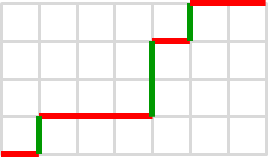
\includegraphics[scale=0.3]{path.png}
    \caption{格路}
\end{figure}
\end{frame}





\begin{frame}{单峰性(unimodality)	}
    	\begin{itemize}
        \item 观察发现任意一行的数字 先单调递增,再单调递减.
    \end{itemize}

    \begin{defi}
        对于序列$s_{0}, s_{1}, \cdots, s_{n}$,如果存在一个整数$t\ (0 \leq t \leq n)$,使得
        $s_{0} \leq s_{1} \leq \cdots \leq s_{t}$,$s_{t}\geq s_{t+1}\geq \cdots \geq s_{n}$
        那么称该序列是单峰的.
    \end{defi}
    \begin{itemize}
        \item  $s_{t}$为该序列的最大数,整数$t$不唯一.
         例如:$1, 3, 3, 1$.
    \end{itemize}
	\begin{thm}
	序列	$\binom{n}{0},\binom{n}{1},\binom{n}{2},\cdots,\binom{n}{n}$是单峰的,
		且最大值是$\binom{n}{\lfloor n/2 \rfloor}=\binom{n}{\lceil n/2 \rceil}.$
	\end{thm}
\pause
提示: 只需对$0\le k \le {\lfloor \frac{n}{2} \rfloor}-1$ 证明
$\binom{n}{k} < \binom{n}{k+1}$.

\end{frame}

%\begin{frame}{对数凹性(logarithmic concave)}
%	\begin{defi}
%		 对于序列$s_{0}, s_{1}, \cdots, s_{n}$,如果存在一个整数$t\ (1 \leq t \leq n-1)$,使得\[
%		 s_{t}^{2}\geq s_{t-1}s_{t+1},
%		 \]则序列$\{s_{t}\}_{0}^{n}$是对数凹的.
%	\end{defi}
%\pause
%\begin{prop}
%	若序列$\{s_{t}\}_{0}^{n}$是对数凹的,则该序列一定是单峰的.
%\end{prop}
%\pause\pf
%反证法.若该序列不是单峰的,则存在连续三项满足\[
%s_{t-1}>s_{t}<s_{t+1}.
%\]于是有$ s_{t}^{2}< s_{t-1}s_{t+1} $,与对数凹性定义矛盾.
%\end{frame}
%
%\begin{frame}
%\begin{prop}
%	二项式系数序列$\{\binom{n}{k}\}_{0}^{n}$是对数凹的.
%\end{prop}
%\pf\textbf{法一(直接证明)}
%
%\[
%\begin{aligned}
%	\frac{\binom{n}{k}^{2}}{\binom{n}{k-1}\binom{n}{k+1}}&=\frac{(\frac{n!}{k!(n-k)!})^{2}}{\frac{n!}{(k-1)!(n-k+1)!}\frac{n!}{(k+1)!(n-k-1)!}}\\
%	&=\frac{(k+1)(n-k+1)}{k(n-k)}\geq1.
%\end{aligned}
%\]故\[
%\binom{n}{k}^{2}\geq \binom{n}{k-1}\binom{n}{k+1},
%\]该序列对数凹.
%\end{frame}
%
%\begin{frame}
%	\textbf{法二(格路组合证明)}
%	\begin{itemize}
%		\item 令$
%		u_1=(1,0), u_2=(0,1), v_1=(k+1, n-k), v_2=(k, n-k+1)$, $p(u_{i};v_{j})$ 表示从 $u_{i}$ 到 $v_{j}$ 只允许向上、向右的格路条数, 于是有
%\[
%p\left(u_1 ; v_1\right)=p\left(u_2 ; v_2\right)=\binom{n}{k},\]
%\[p\left(u_1 ; v_2\right)=\binom{n}{k-1},\quad p\left(u_2 ; v_1\right)=\binom{n}{k+1}.
%\]
%\item 要证\[
%\binom{n}{k}^{2} -\binom{n}{k-1}\binom{n}{k+1}\geq0,
%\]即考虑如下形式$$
%\left|\begin{array}{ll}
%	p\left(u_1 ; v_1\right) & p\left(u_1 ; v_2\right) \\
%	p\left(u_2 ; v_1\right) & p\left(u_2 ; v_2\right)
%\end{array}\right|=p\left(u_1 ; v_1\right) p\left(u_2 ; v_2\right)-p\left(u_1 ; v_2\right) p\left(u_2 ; v_1\right).
%$$
%\item 用$ \mathcal{P}\left(u_i ; v_j\right) $表示从$u_{i}$到$v_{j}$只允许向右、向上的格路集合.
%\item $p\left(u_1 ; v_1\right) p\left(u_2 ; v_2\right)$表示如下格路对的计数
%$$\left(P_1, P_2\right) \in \mathcal{P}\left(u_1 ; v_1\right) \times \mathcal{P}\left(u_2 ; v_2\right):=\mathcal{P}_{12}.$$
%\item 类似地,$ p\left(u_1 ; v_2\right) p\left(u_2 ; v_1\right) $表示如下格路对的计数
%$$
%\mathcal{P}\left(u_1 ; v_2\right) \times \mathcal{P}\left(u_2 ; v_1\right):=\mathcal{P}_{21}.
%$$
%	\end{itemize}
%\end{frame}
%
%\begin{frame}
%
%	 为证明行列式非负,我们要在集合$\mathcal{P}:=\mathcal{P}_{12} \cup \mathcal{P}_{21}$上构建一个符号反转对合$\Omega$,其中符号的定义为
%		$$
%		\operatorname{sgn}\left(P_1, P_2\right)= \begin{cases}+1 & \text { 如果 }\left(P_1, P_2\right) \in \mathcal{P}_{12} \\ -1 & \text { 如果 }\left(P_1, P_2\right) \in \mathcal{P}_{21}\end{cases}
%		$$考虑$\left(P_1, P_2\right)\in \mathcal{P}$,
%		\begin{enumerate}[1]
%			\item 若$P_1 \cap P_2 = \emptyset$, 则该格路对一定属于$ \mathcal{P}_{12} $, 因为$ \mathcal{P}_{21} $中任意路对都相交.此时定义$$
%			\Omega\left(P_1, P_2\right)=\left(P_1, P_2\right).
%			$$
%			\item 若$P_1 \cap P_2 \neq \emptyset$,则考虑路$P_1$ 与 $P_2$的第一个交点 $x$, 定义 $ \Omega\left(P_1, P_2\right)=\left(P_1^{\prime}, P_2^{\prime}\right) $, 其中$$
%			\begin{aligned}
%				&P_1^{\prime}=u_1 \stackrel{P_1}{\rightarrow} x \stackrel{P_2}{\rightarrow} v_2 \\
%				&P_2^{\prime}=u_2 \stackrel{P_2}{\rightarrow} x \stackrel{P_1}{\rightarrow} v_1
%			\end{aligned}
%			$$
%$P_1^{\prime}$ 表示路$ P_1$中从顶点 $u$ 到 $x$ 的部分以及路 $ P_2 $ 中从顶点 $x$ 到 $v_2$ 的部分组成的路, $P_2^{\prime}$类似.
%		\end{enumerate}
%\end{frame}
%
%\begin{frame}
%	\begin{figure}
%		\centering
%		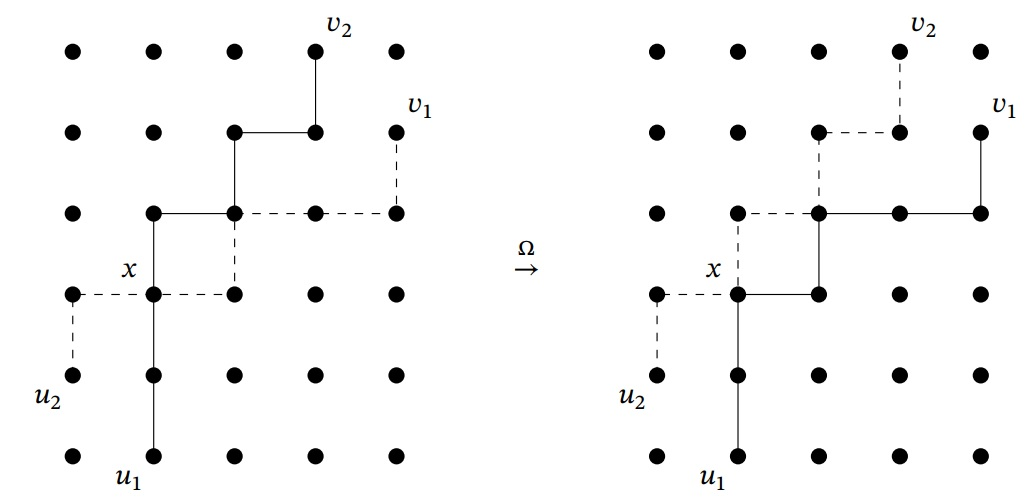
\includegraphics[scale=0.6]{involution.jpg}
%		\caption{符号对合变换}
%	\end{figure}
%由Lindström-Gessel-Viennot引理,有$$
%\left|\begin{array}{ll}
%	p\left(u_1 ; v_1\right) & p\left(u_1 ; v_2\right) \\
%	p\left(u_2 ; v_1\right) & p\left(u_2 ; v_2\right)
%\end{array}\right|=\text { 不相交路对}\left(P_1, P_2\right) \in \mathcal{P}_{12} \text { 条数}.
%$$我们定义其符号为正,因此该行列式为正,即证得二项式系数的对数凹性.
%\end{frame}
%
%\begin{frame}{观察得结论}
%
%	\begin{itemize}
%
%		\item 三角形数: $\binom{n}{2}=\frac{n(n-1)}{2}$
%
%		%\centerline{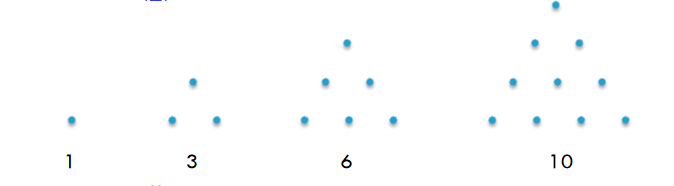
\includegraphics[scale=0.8]{figure3.1.jpg}}
%		%\centerline{三角形阵列点数}
%		\begin{figure}
%			\centering
%			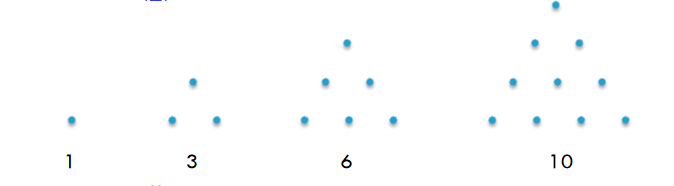
\includegraphics[width=0.7\textwidth]{figure3.1.jpg}
%			\caption{三角形阵列点数}
%		\end{figure}
%
%	\end{itemize}
%\end{frame}
%
%\begin{frame}{观察得结论}
%	\begin{itemize}
%
%	\item 四面体数: $\binom{n}{3}=\frac{n(n-1)(n-2)}{6}$
%%	\centerline{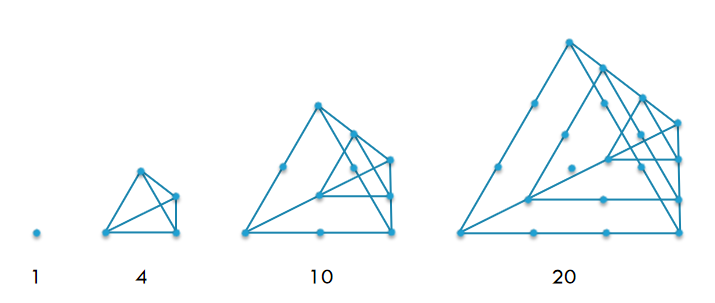
\includegraphics[scale=0.8]{figure3.2.jpg}}
%%	\centerline{四面体阵列点数}
%	\end{itemize}
%	\begin{figure}
%		\centering
%		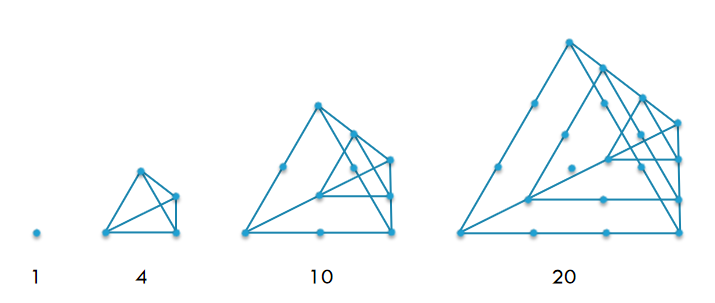
\includegraphics[scale=0.8]{figure3.2.jpg}
%		\caption{四面体阵列点数}
%	\end{figure}
%
%
%\end{frame}
%

%\begin{frame}
%\begin{figure}[H]
%    \centering
%    \begin{subfigure}[b]{0.6\linewidth}
%        \begin{center}
%        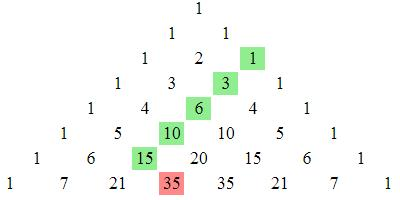
\includegraphics[scale=0.5]{HockeyStick_L.jpeg}
%        \end{center}
%    \end{subfigure}
%    \begin{subfigure}[b]{0.35\linewidth}
%        \begin{center}
%        
\includegraphics[scale=0.25]{HockeyStick.png}
%%            \caption{Hockey stick}
%        \end{center}
%    \end{subfigure}
%
%\end{figure}
%
%%\begin{minipage}{0.65\linewidth}
%%    \begin{figure}
%%        \centering
%%        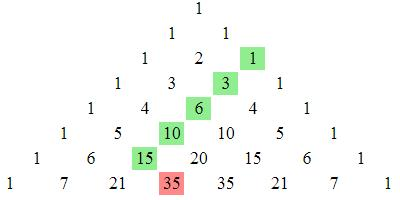
\includegraphics[scale=0.5]{HockeyStick_L.jpeg}
%%    \end{figure}
%%\end{minipage}
%%\begin{minipage}{0.3\linewidth}
%%    \begin{figure}
%%        \centering
%%        
\includegraphics[scale=0.3]{HockeyStick.png}
%%    \end{figure}
%%\end{minipage}
%
%一般地,可以得到
%\begin{block}{朱世杰恒等式}
%设$n,k$是两个正整数.
%若$n>k$, 则
%$$\sum_{i=k}^{n}\binom{i}{k}=\binom{n+1}{k+1}.$$
%\end{block}
%
%一些英文教材上常称这个恒等式为 Hockey-stick identity.
%
%% 提示: 关于$n$做数学归纳法.
%    \end{frame}

\begin{frame}
	\begin{minipage}{0.65\linewidth}
	    \begin{table}[]
	    	\begin{tabular}{c|cccccccc}
	    		$n\backslash k$ & 0 & 1 & 2  & 3  & 4 & 5 & 6 & 7 \\ \hline
	    		0 & 1 &   &    &    &   &   & 	& \\
	    		1 & 1 & 1 &    &    &   &   & 	& \\
	    		2 & 1 & 2 &\cellcolor{green}1  &    &   &   & 	& \\
	    		3 & 1 & 3 & \cellcolor{green}3  & 1  &   &   &	& \\
	    		4 & 1 & 4 & \cellcolor{green}6  & 4  & 1 &   &  & \\
	    		5 & 1 & 5 & \cellcolor{green}10 & 10 & 5 & 1 & & \\
	    		6 & 1 & 6 & \cellcolor{green}15 & 20 & 15 & 6 & 1&  \\
	    		7 & 1 & 7 & 21 & \cellcolor{red}35 & 35 & 21 & 7 & 1\\
	    	\end{tabular}
%	    	\caption{Pascal三角}
	    \end{table}
	\end{minipage}
	\begin{minipage}{0.3\linewidth}
	    \begin{figure}
	        \centering
	        
\includegraphics[scale=0.3]{HockeyStick.png}
	    \end{figure}
	\end{minipage}

	一般地,可以得到
	\begin{block}{朱世杰恒等式}
		设$n,k$是两个正整数.
		若$n>k$, 则
		$$\sum_{i=k}^{n}\binom{i}{k}=\binom{n+1}{k+1}.$$
	\end{block}

	一些英文教材上常称这个恒等式为 Hockey-stick identity.

	% 提示: 关于$n$做数学归纳法.
\end{frame}

%\begin{frame}
%	\begin{table}[]
%		\begin{tabular}{c|cccccccc}
%			$n\backslash k$ & 0 & 1 & 2  & 3  & 4 & 5 & 6 & 7 \\ \hline
%			0 & 1 &   &    &    &   &   & 	& \\
%			1 & 1 & 1 &    &    &   &   & 	& \\
%			2 & 1 & 2 &\cellcolor{green}1  &    &   &   & 	& \\
%			3 & 1 & 3 & \cellcolor{green}3  & 1  &   &   &	& \\
%			4 & 1 & 4 & \cellcolor{green}6  & 4  & 1 &   &  & \\
%			5 & 1 & 5 & \cellcolor{green}10 & 10 & 5 & 1 & & \\
%			6 & 1 & 6 & \cellcolor{green}15 & 20 & 15 & 6 & 1&  \\
%			7 & 1 & 7 & 21 & \cellcolor{red}35 & 35 & 21 & 7 & 1\\
%		\end{tabular}
%		\caption{Pascal三角}
%	\end{table}
%\end{frame}



\begin{frame}
    \begin{ex}
        利用\[m^{2}=2\binom{m}{2}+\binom{m}{1} \]	计算$1^{2}+2^{2}+\cdots+n^{2}$的值.
    \end{ex}
    \pause
    \[
    \begin{aligned}
        1^{2}+2^{2}+\cdots+n^{2}
        &=\sum_{m=1}^{n}m^{2}
        =2\sum_{m=1}^{n}\binom{m}{2}+\sum_{m=1}^{n}\binom{m}{1}\\
        &=2\binom{n+1}{3}+\binom{n+1}{2}\\
        &=\frac{1}{6}n\, (n+1)\, (2n+1).
    \end{aligned}
    \]
\end{frame}


\begin{frame}
    \begin{ex}
        求整数$a,b,c$使得\[m^{3}=a\binom{m}{3}+b\binom{m}{2}+c\binom{m}{1}\tag{*}\]并计算$1^{3}+2^{3}+\cdots+n^{3}$的值.
    \end{ex}
    \pause
    将$m=1,2,3$分别代入(*)式得
    \begin{align*}
        1 = &\,  c \\
        8 = &\,  b+2 c \\
        27 = &\,   a+3 b+3 c
    \end{align*}

    解方程组得$a=6,b=6,c=1$.

\end{frame}

\begin{frame}
    \begin{block}{例}
        求整数$a,b,c$使得\[m^{3}=a\binom{m}{3}+b\binom{m}{2}+c\binom{m}{1}\tag{*}\]并计算$1^{3}+2^{3}+\cdots+n^{3}$的值.
    \end{block}
    \[m^{3}=6\binom{m}{3}+6\binom{m}{2}+\binom{m}{1}\]
    因此,
    \[\begin{aligned}
        1^{3}+2^{3}+\cdots+n^{3} &=\sum_{m=1}^{n} m^{3}
        =6 \sum_{m=1}^{n}\binom{m}{3} +6 \sum_{m=1}^{n} \binom{m}{2}+\sum_{m=1}^{n}\binom{m}{1}\\
        &=6\binom{n+1}{4}+6\binom{n+1}{3}+\binom{n+1}{2} \\
        &=\frac{1}{4} n^{2}(n+1)^{2}
    \end{aligned}\]

\end{frame}

\begin{frame}
清代数学家李善兰(1811-1882)在 《垛积比类》一书中对垛积进行了系统 的研究.所谓垛积数就是二项式系数, 因用于计算按照一定图形堆垛的物品 数量而得其名.在该书的第二卷, 李善兰讨论了如下的求和问题:
$$
1^p+2^p+\cdots+n^p,
$$
其中 $p$ 为正整数.为此他把 $m^p$ 分解成垛积数 $\binom{ m+p-k}{p}$ 的线性组合
$$
m^p=\sum_{k=1}^p A(p, k) \binom{ m+p-k}{p}, \quad m=1,2, \ldots, n,
$$
其中 $A(p, k)$ 为与 $m$ 无关的系数, 称为李善兰系数.

闻名中外的 “李善兰恒等 式” 就是从上述分解过程中归纳得到的:
$$
\sum_{k=0}^m \binom{m}{k}^2
    \binom{n+2 m-k}{2 m}
=\binom{m+n
}{n}^2 .
$$

Andrews 称上述恒等式为中国恒等式(Chinese Identity).

华罗庚给 出了这个恒等式的数学归纳法证明.
\end{frame}

\section{二项式定理}
\begin{frame}{二项式定理}
	\begin{thm}
		令$n$是一个正整数,对所有的$x$和$y$,有
		$$(x+y)^{n}=\sum _{k=0}^n  \binom{n}{k} x^{n-k}y^k.$$
	\end{thm}

	\begin{itemize}

		\item 证明一:乘法分配律展开,再合并同类项.\\
将$(x+y)^n$写作$$(x+y)^n=\underbrace{(x+y) \cdot(x+y) \cdot(x+y) \cdots \cdot(x+y)}_n,$$
我们发现对于$x^{n-k}y^k$一项,一定有$n$项乘积中的$n-k$项贡献了$x$,其余$k$项贡献了$y$.因此$x^{n-k}y^k$项系数为$\binom{n}{k}$.
		\item 证明二:归纳法.


	\end{itemize}

\end{frame}
\begin{frame}{二项式定理}
	 证明三:泰勒级数展开.\\
	$e^x$的泰勒级数为$$\sum_{n=0}^{\infty}\frac{x^n}{n!}=1+x+\frac{x^2}{2}+\frac{x^3}{6}+\cdots.$$
	因为$e^{x+y}=e^x e^y$,相同函数的幂级数逐项相等,于是在$x+y$处的级数等于在$x$处的级数和在$y$处的级数的卷积,即
	$$\frac{(x+y)^n}{n!}=\sum_{k=0}^{n}\frac{x^{n-k}}{(n-k)!}\frac{y^k}{k!},$$化简得$$(x+y)^{n}=\sum_{k=0}^{n}\frac{n!}{k!(n-k)!}x^{n-k}y^k=\sum _{k=0}^n  \binom{n}{k} x^{n-k}y^k.$$

\end{frame}

\begin{frame}{等价形式}
\begin{itemize}
    \item $(x+y)^{n}=\sum\limits_{k=0}^n  \binom{n}{k} x^{n-k} y^k$
	\item $(x+y)^{n}=\sum\limits_{k=0}^n  \binom{n}{n-k} x^{n-k} y^k$

	\item $(x+y)^{n}=\sum\limits_{k=0}^n  \binom{n}{n-k} x^k y^{n-k}$

	\item $(x+y)^{n}=\sum\limits_{k=0}^n  \binom{n}{k} x^k y^{n-k}$
\end{itemize}
	特殊地, 令$y=1$,得
\begin{cor}
令$n$是一个正整数,对所有的$x$,有
$$(1+x)^{n}=\sum _{k=0}^n  \binom{n}{k} x^k=\sum _{k=0}^n  \binom{n}{n-k} x^k$$
\end{cor}

\end{frame}


\begin{frame}
    \begin{ex}
        用二项式定理展开$(2x-y)^{4}$.
    \end{ex}

    \begin{ex}
        $(3x-2y)^{9}$的展开式中,  $x^{2}y^{7}$的系数是什么?$x^{7}y^{2}$的系数是什么?
    \end{ex}


    \pause
    \[\begin{aligned}
        (2x-y)^{4}&=16 x^4-32 x^3 y+24 x^2 y^2-8 x y^3+y^4.
    \end{aligned}
    \]


    \[
    (3x-2y)^{9}=\sum_{r=0}^{9}\binom{9}{r}(3x)^{r}(-2y)^{9-r}
    \]

\begin{center}
$x^{2}y^{7}$系数:$\binom{9}{2}3^{2}(-2)^{7} = -41472$

$x^{7}y^{2}$系数:$\binom{9}{7}3^{7}(-2)^{2} = 314928$
\end{center}

\end{frame}






%\section{牛顿二项式定理}



\begin{frame}{牛顿二项式定理}
	\begin{defi}
    设$\alpha$是实数,$k$是非负整数,定义二项式系数为\vspace*{8pt}
    $$
    \binom{\alpha}{k}=\left\{\begin{array}{cc}
        \frac{\alpha({\alpha}-1) \cdots(\alpha-{k}+{1})}{{k} !} & {k} \geq {1}
       \\[6pt]
        {1} & {k}={0}
%        \\[6pt]
%        {0} & {k} < 0
    \end{array}\right.
    $$
\end{defi}

	\begin{thm}
	设$\alpha$是实数,对$|z|< 1$的$z$,有
		$$(1+z)^{\alpha}=\sum _{k=0}^\infty \binom{\alpha}{k} z^k$$
%		其中$\binom{\alpha}{k}=\frac{\alpha (\alpha -1)\cdots(\alpha-k+1)}{k!}$
	\end{thm}

\end{frame}

\begin{frame}{常用展开式}
	\begin{itemize}
	\item $ \alpha = -n$,其中$n$为正整数
	\end{itemize}
$$
\begin{aligned}
    \binom{-n}{k}
    &=\frac{(-n)(-n-1) \cdots(-n-k+1)}{k !} \\
    &=(-1)^{k} \frac{n(n+1) \cdots(n+k-1)}{k !} \\
    &=(-1)^{k} \binom{n+k-1}{k}
\end{aligned}
$$
因此
$$(1+z)^{-n}=\sum_{k=0}^\infty (-1)^k \binom{n+k-1}{k} z^k$$
\end{frame}

\begin{frame}
    \begin{itemize}
        \item $(1+z)^{-n}=\sum\limits_{k=0}^\infty (-1)^k \binom{n+k-1}{k} z^k$
        \item $(1+z)^{-1}=\sum\limits_{k=0}^\infty (-1)^k z^k$
        \item  $(1+z)^{-2}=\sum\limits_{k=0}^\infty (-1)^k (k+1) z^k$
    \end{itemize}


    令$-z$代替上面的$z$

    \begin{itemize}
        \item $(1-z)^{-n}=\sum\limits_{k=0}^\infty  \binom{n+k-1}{k} z^k$
        \item $(1-z)^{-1}=\sum\limits_{k=0}^\infty  z^k$
        \item  $(1-z)^{-2}=\sum\limits_{k=0}^\infty (k+1) z^k$
    \end{itemize}
    \begin{cor}
    $(1-z)^{-n}$中$z^k$的系数等于$k_1+k_2+ \cdots +k_n=k$的非负整数解,即  $\binom{n+k-1}{k}$.
\end{cor}

\vspace{-15pt}
    \begin{align*}
        (1-z)^{-n} & =(1-z)^{-1} \cdots (1-z)^{-1}  =(1+z+z^2+\cdots)\cdots(1+z+z^2+\cdots)
    \end{align*}

    从第一个因子选取$z^{k_1}$,从第二个因子选取$z^{k_2},\cdots$


\end{frame}


\begin{frame}{常用展开式}
    	\begin{itemize}
        \item $ \alpha = 1/2$
    \end{itemize}
\begin{align*}
\binom{1/2}{k}
= & \frac{\left(\frac{1}{2}\right)\left(\frac{1}{2}-1\right) \cdots\left(\frac{1}{2}-k+1\right)}{k !}\\[6pt]
= & \frac{(-1)^{k-1} \cdot 1 \cdot 1 \cdot 3 \cdots(2 k-3)}{2^{k} \cdot k !} \\[6pt]
=& \frac{(-1)^{k-1} \cdot(2 k-3) ! ! \cdot(2 k-2) ! !}{2^{k} \cdot k ! \cdot(2 k-2) ! !}\\[6pt]
= & \frac{(-1)^{k-1} \cdot(2 k-2) !}{2^{2 k-1} \cdot k ! \cdot(k-1) !} \\[6pt]
= & \frac{(-1)^{k-1}}{2^{2 k-1} \cdot k}
\binom{2 k-2}{k-1}
\end{align*}

%	对 $|{z}|<1, $ 有
因此
\vspace{-10pt}
    $$(1+z)^{1 / 2}=1+\sum_{k=1}^{\infty} \frac{(-1)^{k-1}}{2^{2 k-1} \cdot k}\left(\begin{array}{c}2 k-2 \\ k-1\end{array}\right) z^{k}$$
%	$$
%	=1+\frac{1}{2} z-\frac{1}{2 \cdot 2^{3}}\left(\begin{array}{l}
%	2 \\ 1
%	\end{array}\right) z^{2}+\frac{1}{2 \cdot 2^{5}}\left(\begin{array}{l}
%	4 \\ 2
%	\end{array}\right) z^{3}-\cdots
%	$$



\end{frame}




\section{多项式定理}

\begin{frame}{回顾——重集的排列数}
	\begin{thm}
		令$S$是一个有$t$个不同类型的元的多重集,各个元的重数分别为$n_{1}, n_{2}, \cdots, n_{t}$,
		满足$n=n_{1}+ n_{2}+\cdots+ n_{t}$,则$S$的排列数等于
		$$
		\frac{n!}{n_{1}!n_{2}!\cdots n_{t}!}
		$$
	\end{thm}

	\begin{defi}
	多项式系数定义为
	$$
	\binom{n}{n_{1}, n_{2}, \cdots, n_{t}}=\frac{n!}{n_{1}!n_{2}!\cdots n_{t}!}
	$$
	这里$n=n_{1}+ n_{2}+\cdots+ n_{t}$.
	\end{defi}
\end{frame}

\begin{frame}{多项式定理}
	\begin{thm}
	对于$t$个不同的变量$x_{1}, x_{2}, \cdots, x_{t}$有
	$$
	\left(x_{1}+x_{2}+\cdots+x_{t}\right)^{n}=\sum_{n_{1}+n_{2}+\cdots+n_{t}=n, \atop n_{1}, n_{2}, \cdots, n_{t} \geqslant 0}\left(\begin{array}{c}
	n \\ n_{1}, n_{2}, \cdots, n_{t}
	\end{array}\right) x_{1}^{n_{1}} x_{2}^{n_{2}} \cdots x_{t}^{n_{t}}
	$$

	\end{thm}
	\begin{itemize}
	\item  证明:利用乘法的分配律将乘积完全展开,再考虑合并同类项,
	$x_{1}^{n_{1}} x_{2}^{n_{2}} \cdots x_{t}^{n_{t}}$有$\binom{n}{n_{1}, n_{2}, \cdots, n_{t}}$种排列.

	\end{itemize}

\end{frame}


\begin{frame}{多项式定理}


	\begin{ex}
		展开式$(2x_{1}-3x_{2}+5x_{3})^6$中, $x_{1}^{3}x_2x_3^2$的系数是多少?
	\end{ex}

	\begin{ex}
    确定$\left(x_{1}+x_{2}+x_{3}+x_{4}+x_{5}\right)^{10}$的展开式中$ x_{1}^{3} x_{2} x_{3}^{4} x_{5}^{2}$项的系数.
\end{ex}


\pause
		$$
		\left(\begin{array}{c}
		6 \\ 3,1,2
		\end{array}\right) 2^{3}(-3)^{1} 5^{2}=-36000
		$$

\pause
\[\left(\begin{array}{c}
    10 \\
    3,1,4,2
\end{array}\right)=\frac{10 !}{3 ! 1 ! 4 ! 2 !}=12600\]


\end{frame}

\begin{frame}{多项式定理}

	\begin{ex}
		展开式 $\left(x_{1}+x_{2}+\cdots+x_{t}\right)^{n}$ 中,共有多少不同的项?
	\end{ex}
	\pause

		展开式中,一般项为 $x_{1}^{n_{1}} x_{2}^{n_{2}} \cdots x_{t}^{n_{t}}$, 满足 $$n_{1}+n_{2}+\cdots+n_{t}=n$$
		因此不同的项的数目等同于上述方程的非负整数解 的个数,即 $\binom{n+t-1}{n}.$

\end{frame}




\section{组合恒等式}
\begin{frame}{组合恒等式}
	\begin{iden}
		$$
	\sum_{k=0}^n \binom{n}{k}=2^{n}
		$$
	\end{iden}
	%$\boldsymbol{i)}$ $\binom{n}{0}+\binom{n}{1}+\cdots+\binom{n}{n}=2^{n}$
   \pause
	\begin{itemize}
	\item 对应着二项式定理中:$x = 1$,$y = 1$;
	\item 如果$S$是$n$个元素的集合,则$S$的所有组合有多少个?
	\end{itemize}
\end{frame}

\begin{frame}
	\begin{iden}设 $n \geq 1$, 则
	$$
	\sum_{k=0}^n (-1)^k \binom{n}{k}=0
	$$
	\end{iden}
\pause
	\begin{itemize}
    \item 对应着二项式定理中:$x = 1,y = -1$
    \item $S$的具有偶数个元素的组合有多少个?具有奇数个元素的组合有多少个?
    \item 可否建立奇组合与偶组合之间的一一对应?
\end{itemize}
\end{frame}

\begin{frame}
\begin{block}{推论}
设 $n \geq 1$, 则
$$
\sum_{k \text { 为奇数 }}\binom{n}{k} =\sum_{k \text { 为偶数 }}  \binom{n}{k}
$$
\end{block}
%下面给出推论 $1.4 .5$ 的一个不依赖性质 $1.4 .4$ 的组合证明.


证明\quad  设 $X=\{1,2, \ldots, n\}$, 则
\begin{align*}
A& =\{S \subseteq X  : \, | S| \, \mbox{为偶数且} 1 \in S\}, \\
B&=\{S \subseteq X  : \,| S| \, \mbox{为奇数且} 1 \in S\},\\
C&=\{S \subseteq X  : \, | S| \, \mbox{为偶数且} 1 \notin S\},\\
D& =\{S \subseteq X  :  \,| S| \,  \mbox{为奇数且} 1 \notin S\}.
\end{align*}


 构造映射 $f: A \rightarrow D$ 为 $f\, (S)=S  \, \backslash\{1\}$, 显然 $f$ 为双射.
  所以 $|A|=|D|$.

 类似地 $|B|=|C|$.

  因此
$$
\sum_{k \text { 为奇数 }}\binom{n}{k}
=|B|+|D|=|C|+|A|
=\sum_{k \text { 为偶数 }}\binom{n}{k}.
$$

\end{frame}



\begin{frame}

    \begin{iden}\label{eq:nk}
对于正整数$n,k,$
        $$
        k \binom{n}{k}=n\binom{n-1}{k-1}.
        $$
    \end{iden}
    \pause
\begin{itemize}
        %	\item 从$n$个人中挑选$k$个人组成一个队,并选择一人为队长,有多少种方法?
        \pause

\item
        %    (组合证明)即证$k\binom{n}{k}=n\binom{n-1}{k-1}$.
        考虑从$n$人中选出带队长的$k$人小队:

\item  可先从$n$人中选出$k$人做队员,再从$k$人中选出一人做队长;


\item 也可以从$n$人中选出一人做队长,然后再从$n-1$人中选出$k-1$人做队员.

    \end{itemize}

\end{frame}


\begin{frame}
    \begin{ex}
        利用 $k \binom{n}{k}=n\binom{n-1}{k-1}$ 计算
        \begin{enumerate}
            \item
            $\sum\limits_{k=1}^{n} k\binom{n}{k} $
            \item
            $\sum\limits_{k=2}^{n} k(k-1)\binom{n}{k}$

            %		$(3)\sum_{k=1}^{n} k^{2}\binom{n}{k}$
            \item
            $\sum\limits_{k=0}^{n} \frac{1}{k+1}\binom{n}{k}$
        \end{enumerate}
    \end{ex}

    \pause
    % \textbf{解}\quad
    \begin{enumerate}
        \item  $\quad  \sum\limits_{k=1}^{n} k \binom{n}{k}
        =\sum\limits_{k=1}^{n} k \cdot \frac{n}{k}\binom{n-1}{k-1}
        =n \sum\limits_{k=1}^{n} \binom{n-1}{k-1}=n \sum\limits_{i=0}^{n-1} \binom{n-1}{i}=n  2^{n-1}.$

        \item
        $\quad \sum\limits_{k=2}^{n} k(k-1) \binom{n}{k}
        =n \sum\limits_{k=2}^{n}(k-1)  \binom{n-1}{k-1}=n \sum\limits_{k=1}^{n-1} k  \binom{n-1}{k}
        =n (n-1)  2^{n-2}.$

        %    \item  利用前两个式子证明.
        \item
        %    最后一个式子
        %    可用 $\binom{n}{k}=\frac{n}{k}\binom{n-1}{k-1}$ 这个公式证明.

        $\quad  \sum\limits_{k=0}^{n} \frac{1}{k+1}\binom{n}{k}=\sum_{k=0}^{n} \frac{1}{n+1}\binom{n+1}{k+1}=\frac{1}{n+1} \sum\limits_{k=1}^{n+1}\binom{n+1}{k}$\\[6pt]
        $=\frac{1}{n+1}\left(\sum\limits_{k=0}^{n+1}\binom{n+1}{k} -\binom{n+1}{0}\right)=\frac{2^{n+1}-1}{n+1}.$
    \end{enumerate}

\end{frame}




\begin{frame}
	\begin{iden}
        对于正整数$n$
		$$\sum_{k=1}^{n} k\binom{n}{k}=n 2^{n-1}.$$
	\end{iden}
	\pause
方法1: 对$\sum _{k=0}^n  \binom{n}{k}x^{k}=(1+x)^{n}$两边同时求导得
		$$\sum _{k=0}^n  k\binom{n}{k}x^{k-1}=n(1+x)^{n-1},$$再令$x=1$.

方法2: 应用等式\, \ref{eq:nk}   $$\sum _{k=1}^n  k\binom{n}{k}=\sum _{k=1}^n  n\binom{n-1}{k-1}=n2^{n-1}.$$

方法3: 从$n$个人中挑选$k\ (k=1, 2, \cdots, n)$个人组成一个队,并选择一人为队长,有多少种方法?

\end{frame}



\begin{frame}
\begin{iden}\label{eq:kk}
对于整数$n \ge 2,$
    $$\sum_{k=1}^{n} k^{2}\binom{n}{k}=n(n+1) 2^{n-2}.$$
\end{iden}
	\pause
	\textbf{ 证明 } \quad  对$(1+x)^{n}=\sum_{k=0}^{n}\binom{n}{k}x^{k}$求导, 得
    \[n(1+x)^{n-1}=\sum_{k=1}^{n}k\binom{n}{k}x^{k-1}.\]
	将上式左右两边同乘$x$, 得
    \[
	nx(1+x)^{n-1}=\sum_{k=1}^{n}k\binom{n}{k}x^{k}.
	\]
	对上式左右两边\blue{求导}, 得
    \[
	n\left((1+x)^{n-1}+(n-1) x(1+x)^{n-2} \right)=\sum_{k=1}^{n} k^{2}\binom{n}{k} x^{k-1}.
	\]
	令$x=1$, 得
    \[
	\sum_{k=1}^{n} k^{2}\binom{n}{k} =n\left(  2^{n-1}+(n-1) 2^{n-2}   \right)=n(n+1) 2^{n-2}.
	\]

\end{frame}

\begin{frame}
\begin{block}{恒等式\, \ref{eq:kk}}
对于整数$n \ge 2,$
		$$\sum_{k=1}^{n} k^{2}\binom{n}{k}=n(n+1) 2^{n-2}.$$
\end{block}

	\begin{itemize}

	\item 从$n$个人中挑选$k\ (k=1, 2, \cdots, n)$个人组成一个班级,并选择班长、团支书各一人(可兼任),有多少种方法?
    \pause
\item $n(n-1)2^{n-2}+n 2^{n-1}=n(n+1) 2^{n-2}.$
	\end{itemize}
\end{frame}


\begin{frame}
	\begin{iden}
		证明等式$$\sum_{k=0}^{n} \frac{1}{k+1} \binom{n}{k}   =\frac{2^{n+1}-1}{n+1}.$$
	\end{iden}
	\pause
	\textbf{ 证明 } \quad 对
	$$
(1+x)^{n}=\sum_{k=0}^{n}\binom{n}{k} x^{k},
	$$
	两边对 $x$ 求从 0 到 1 的\blue{定积分},
	\begin{align*}
		\int_{0}^{1}(1+x)^{n} \mathrm{~d} x & =\sum_{k=0}^{n}\binom{n}{k} \int_{0}^{1} x^{k} \mathrm{~d} x, \\
		\left.\frac{1}{n+1}(1+x)^{n+1}\right|_{0} ^{1} & =\left.\sum_{k=0}^{n}\binom{n}{k} \cdot \frac{1}{k+1} x^{k+1}\right|_{0} ^{1}, \\
		\frac{1}{n+1}\left(2^{n+1}-1\right) & =\sum_{k=0}^{n} \frac{1}{k+1}\binom{n}{k}.
	\end{align*}
	此即所证等式.


%注:使用这种方法证明恒等式时一定要取定积分,否则易出现常数确定上的错误.
\end{frame}

\begin{frame}
    \begin{minipage}{0.65\linewidth}
        \begin{table}[]
            \begin{tabular}{c|cccccccc}
                $n\backslash k$ & 0 & 1 & 2  & 3  & 4 & 5 & 6 & 7 \\ \hline
                0 & 1 &   &    &    &   &   & 	& \\
                1 & 1 & 1 &    &    &   &   & 	& \\
                2 & 1 & 2 &\cellcolor{green}1  &    &   &   & 	& \\
                3 & 1 & 3 & \cellcolor{green}3  & 1  &   &   &	& \\
                4 & 1 & 4 & \cellcolor{green}6  & 4  & 1 &   &  & \\
                5 & 1 & 5 & \cellcolor{green}10 & 10 & 5 & 1 & & \\
                6 & 1 & 6 & \cellcolor{green}15 & 20 & 15 & 6 & 1&  \\
                7 & 1 & 7 & 21 & \cellcolor{red}35 & 35 & 21 & 7 & 1\\
            \end{tabular}
            %	    	\caption{Pascal三角}
        \end{table}
    \end{minipage}
    \begin{minipage}{0.3\linewidth}
        \begin{figure}
            \centering
            
\includegraphics[scale=0.3]{HockeyStick.png}
        \end{figure}
    \end{minipage}

    一般地,可以得到
    \begin{block}{朱世杰恒等式}
        设$n,k$是两个正整数.
        若$n>k$, 则
        $$\sum_{i=k}^{n}\binom{i}{k}=\binom{n+1}{k+1}.$$
    \end{block}

    一些英文教材上常称这个恒等式为 Hockey-stick identity.


\end{frame}

\begin{frame}

    \begin{iden}[朱世杰恒等式]
        设$n,k$是两个正整数.
        若$n>k$, 则	$$\sum_{i=k}^{n}\binom{i}{k}=\binom{n+1}{k+1}.$$
    \end{iden}
    \pause
       归纳法证明:关于$n$做归纳.

    组合证明:
    \begin{itemize}
        \item 从$n+1$个人中挑选$k+1$个人组成一个队.
        \item 先从$n+1$个人当中挑出一个人,令他的号码是$i+1\ (i= k, \cdots, n)$,
        作为小队当中号码最大的人.

        \item 接下来只要从前$i$个人当中挑出剩下的$k$个人即可.
    \end{itemize}

    比较系数法:
    提取 $$\sum_{i=0}^{n}(1+x)^{i}= \frac{(1+x)^{n+1}-1}{x}$$ 两边 $x^{k}$ 的系数.
\end{frame}



\begin{frame}
    \begin{block}{朱世杰恒等式}
        %    设$n,k$是两个正整数.
        %    若$n>k$, 则
        $$\sum_{i=k}^{n}\binom{i}{k}=\binom{n+1}{k+1}$$
    \end{block}
%  机器证明:
  利用
%    临差算子
    $$
    \binom{i}{k} =  \binom{i+1}{k+1}-\binom{i}{k+1}
    $$
    可知
    $$
    \begin{aligned}
        \sum_{i=k}^{n}\binom{i}{k}
        &=\sum_{i=k}^{n}\left( \binom{i+1}{k+1}-\binom{i}{k+1}\right) \\
        &=\sum_{i=k}^{n}\binom{i+1}{k+1}  -\sum_{i=k}^{n}\binom{i}{k+1} \\
        &=\sum_{\blue{i=k+1}}^{\blue{n+1}}\binom{\blue{i}}{k+1}-\sum_{i=k}^{n}\binom{i}{k+1} \\
        &=\binom{n+1}{k+1}-\underbrace{\binom{k}{k+1}}_{0}
        =\binom{n+1}{k+1}
    \end{aligned}
    $$
\end{frame}
\begin{frame}
%    {不定和}
    对于$f(i)$, 如果存在它的\blue{差分}$F(i)$满足
    $$\Delta_i F(i) =F(i+1)-F(i)=f(i),$$
    则称$F(i)$是$f(i)$的\blue{不定和}.
    于是
    $$
        \sum_{i=a}^{b} f(i) =\sum_{i=a}^{b}  F(i+1)-\sum_{i=a}^{b}  F(i) =F(b+1)-F(a).
    $$


       \alert{Gosper算法}:

        输入:超几何项$f(i)$,也就是$f(i+1)/f(i)$是有理函数.

        输出:
        \begin{itemize}
            \item $F(i)$ 使得$\Delta_i F(i)=F(i+1)-F(i)=f(i)$;
           \item   算法失败,若满足条件的超几何项$g(i)$不存在.
        \end{itemize}

    Gosper算法适用于求下面的不定和
\begin{align*}
    \sum_{i=0}^{n}\frac{\binom{2i}{i}^2}{(i+1)4^{2i}}=\sum_{i=0}^{n}\Delta_i \frac{4i\binom{2i}{i}^2}{4^{2i}}=\frac{(n+1)\binom{2n+2}{n+1}^2}{4^{2n+1}}.
\end{align*}

\end{frame}

\begin{frame}
%    给定数列$f(n)$,寻找另一数列$g(n)$使得
%    $$\sum_{k=0}^{n-1}f(k)=g(n)\Leftrightarrow f(n)=g(n+1)-g(n).$$
%    多项式总是可求和的
%    $$\binom{k}{m}=\Delta_k \binom{k}{m+1}=\binom{k+1}{m+1}-\binom{k}{m+1}.$$



不定和没有好的表达式,定和可能有好的表达式.

例如$\binom{n}{i}$
关于 $i$ 的不定和不是超几何的,但是
    $$\sum_{i=0}^{n}\binom{n}{i}=2^n.$$

处理定和问题的基本方法是
\begin{center}
\alert{构造和式满足的多项式系数的递推关系.}
\end{center}

\end{frame}



\begin{frame}

    \begin{block}{朱世杰恒等式}
        %    设$n,k$是两个正整数.
        %    若$n>k$, 则
        $$\sum_{i=k}^{n}\binom{i}{k}=\binom{n+1}{k+1}$$
    \end{block}



    \begin{minipage}{0.45\linewidth}
        \begin{figure}
            \centering
            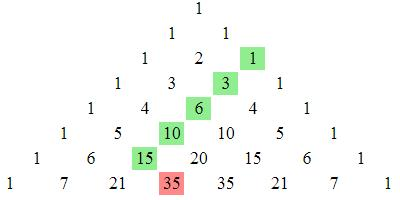
\includegraphics[scale=0.4]{HockeyStick_L.jpeg}
        \end{figure}
    \end{minipage}
    \hspace{10pt}
    \begin{minipage}{0.45\linewidth}
        \begin{figure}
            \centering
            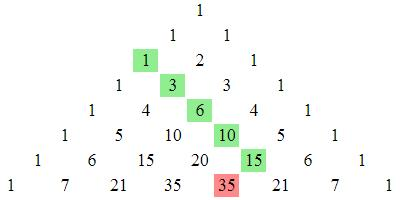
\includegraphics[scale=0.4]{HockeyStick_R.jpeg}
        \end{figure}
    \end{minipage}


    \begin{iden}
        $$\sum_{i=0}^{k}\binom{n+i}{i}=\binom{n+k+1}{k}$$
    \end{iden}
\end{frame}


%
%\begin{frame}
%
%	\begin{block}{朱世杰恒等式}
    %		%    设$n,k$是两个正整数.
    %		%    若$n>k$, 则
    %		$$\sum_{i=k}^{n}\binom{i}{k}=\binom{n+1}{k+1}$$
    %	\end{block}
%	\begin{minipage}{0.3\linewidth}
    %		\begin{table}[]
        %			\begin{tabular}{c|cccccccc}
            %				$n\backslash k$ & 0 & 1 & 2  & 3  & 4 & 5 & 6 & 7 \\ \hline
            %				0 & 1 &   &    &    &   &   & 	& \\
            %				1 & 1 & 1 &    &    &   &   & 	& \\
            %				2 & 1 & 2 &\cellcolor{green}{1}  &    &   &   & 	& \\
            %				3 & 1 & 3 & \cellcolor{green}3  & 1  &   &   &	& \\
            %				4 & 1 & 4 & \cellcolor{green}6  & 4  & 1 &   &  & \\
            %				5 & 1 & 5 & \cellcolor{green}10 & 10 & 5 & 1 & & \\
            %				6 & 1 & 6 & \cellcolor{green}15 & 20 & 15 & 6 & 1&  \\
            %				7 & 1 & 7 & 21 & \cellcolor{red}35 & 35 & 21 & 7 & 1\\
            %			\end{tabular}
        %		\end{table}
    %	\end{minipage}
%	\hspace{10pt}
%	\begin{minipage}{0.4\linewidth}
    %		\begin{tabular}{c|cccccccc}
        %			\resizebox{0.4\columnwidth}
        %			$n\backslash k$ & 0 & 1 & 2  & 3  & 4 & 5 & 6 & 7 \\ \hline
        %			0 & 1 &   &    &    &   &   & 	& \\
        %			1 & 1 & 1 &    &    &   &   & 	& \\
        %			2 & \cellcolor{green}1 & 2 &1  &    &   &   & 	& \\
        %			3 & 1 & \cellcolor{green}3 &3  & 1  &   &   &	& \\
        %			4 & 1 & 4 & \cellcolor{green}6  & 4  & 1 &   &  & \\
        %			5 & 1 & 5 &10 & \cellcolor{green}10 & 5 & 1 & & \\
        %			6 & 1 & 6 &15 & 20 & \cellcolor{green}15 & 6 & 1&  \\
        %			7 & 1 & 7 & 21 &35 & \cellcolor{red}35 & 21 & 7 & 1\\
        %		\end{tabular}
    %
    %	\end{minipage}
%
%	\begin{iden}
    %	$$\sum_{i=0}^{k}\binom{n+i}{i}=\binom{n+k+1}{k}$$
    %	\end{iden}
%\end{frame}








\begin{frame}
	\begin{iden}[范德蒙恒等式]\label{eq:V}
        若$m, n$是正整数, $k$是非负整数, 则
	$$
    \sum_{i=0}^{k}
    \binom{m}{i}
    \binom{n}{k-i} = \binom{m+n}{k}.$$
	\end{iden}

\pause


方法1:  比较等式 $(x+1)^{m+n}=(x+1)^{m}(x+1)^{n}$ 两边 $x^{k}$ 的系数.

方法2:
\begin{itemize}
\item   $\binom{m+n}{k}$ 是 $(m+n)$元集合$A \cup B$ 中 $k$-子集的个数, 其中 $A=\{1, \ldots, m\}, B=\{m+1, \ldots, m+n\}$,
\item 而其中包含 $A$ 中 $i$ 个元素的这样的 $k$-子集的个数 为 $\binom{m}{i}
\binom{n}{k-i}$,
\item  所以和式 $\sum_{i=0}^{m}\binom{m}{i}
\binom{n}{k-i}$ 便是对所有的 $i$ 来计这些子集的个数.

\end{itemize}
特别地, 当$m=n=k$时,
\begin{block}{推论}
%    {范德蒙恒等式}
    $$\sum_{i=0}^{n}\binom{n}{i}^{2}=\binom{2n}{n}.$$
\end{block}
\end{frame}

\begin{frame}

方法3:机器证明.

 Doron Zeilberger提出了一种证明组合恒等式(更一般的“超几何恒等式”)的机械化算法. 他认识到问题的实质是:为证明恒等式
$$\sum_k f(n,k)=g(n),$$
只需:
\begin{itemize}
    \item 找出一个左边和式$F(n)=\sum_k f(n,k)$满足的递推关系;
    \item 用代入的方法验证右边$g(n)$也满足同样的递推关系;
    \item 用足够多的初始值验证等式两边相等.
\end{itemize}
因此寻找和式的递推关系就成了证明和发现恒等式的首要任务.


例如
	$$\sum_{k=0}^n \binom{n}{k}=2^{n}$$
\end{frame}


\begin{frame}{Zeilberger算法}



        输入:
        双超几何项$f(n,i)$, 即$f(n+1,i)/f(n,i)$以及$f(n,i+1)/f(n,i)$均为关于$n$和$i$的有理函数.


        输出:
        \begin{itemize}
            \item 邻差算子$$L=\sum_{j=0}^{d}a_j(n)S_n^{\, j},$$ 其中 $S_n f(n, i)= f(n+1, i)$ 和

            \item 超几何项$g(n,i)$使得
             $$L(f)=\Delta_i g(n,i) =g(n,i+1)-g(n,i).$$
             于是,
            $$a_0(n)f(n,i)+a_1(n)f(n+1,i)+\cdots+a_d(n)f(n+d,i)=g(n,i+1)-g(n,i).$$

        \end{itemize}

   若邻差算子$L$不存在,则算法失效.


\end{frame}

\begin{frame}{Zeilberger算法证明组合恒等式}
\begin{block}{范德蒙恒等式}
    若$m,n$是正整数,则
	$$
    \sum_{i=0}^{k}
    \binom{m}{i}
    \binom{n}{k-i} = \binom{m+n}{k}.$$
\end{block}

令$f(n,i)=\binom{m}{i}\binom{n}{k-i}$及$F(n)=\sum_{i=0}^{k}f(n,i)$, Zeilberger算法可以找到
$$L=(m+n-k+1)S_n-(m+n+1), \quad g(n,i)=i\binom{m}{i}\binom{n}{k-i},$$
即
$$(m+n-k+1)f(n+1,i)-(m+n+1)f(n,i)=g(n,i+1)-g(n,i).$$
%$$(m+n-k+1)f(n+1,i)-(m+n+1)f(n,i)=\Delta_i(g)$$
对$i$从$0$到$k$求和可得
$$\alert{(m+n-k+1)F(n+1)-(m+n+1)F(n)=g(n,k+1)-g(n,0)=0}.$$
最后需要验证$\binom{m+n}{k}$满足与$F(n)$有相同的\blue{初值}和\blue{递推关系}.
\end{frame}

\begin{frame}{Zeilberger算法证明组合恒等式}
    \begin{block}{范德蒙恒等式}
        若$m,n$是正整数,则
        $$
        \sum_{i=0}^{k}
        \binom{m}{i}
        \binom{n}{k-i} = \binom{m+n}{k}.$$
    \end{block}


等号左边$F(n)=\sum_{i=0}^{k}\binom{m}{i}\binom{n}{k-i}$的\blue{初值}为${F(0)=\binom{m}{k}}$, \blue{递推关系}为
    $${(m+n-k+1)F(n+1)=(m+n+1)F(n)}.$$

等号右边$\binom{m+n}{k}$的\blue{初值}为${\binom{m+0}{k} = \binom{m}{k}}$, \blue{递推关系}为
$${(m+n-k+1)\binom{m+n+1}{k}=(m+n+1)\binom{m+n}{k}}.$$
因此, $F(n)$与 $\binom{m+n}{k}$具有相同的{初值}和{递推关系}.
\end{frame}

 \begin{frame}

        \begin{block}{范德蒙恒等式}
         若$m,n$是正整数,则
         $$
         \sum_{i=0}^{k}
         \binom{m}{i}
         \binom{n}{k-i} = \binom{m+n}{k}$$
     \end{block}
     Mathematica代码实现:
     \begin{mma}
         \In <<RISC ~\grave{ } \, fastZeil~\grave{}
         \linebreak
         \text{Fast Zeilberger Package version 3.61}
         \linebreak
         \text{written by Peter Paule, Markus Schorn, and Axel Riese}
         \linebreak
         \text{Copyright Research Institute for Symbolic Computation (RISC),}
         \linebreak
         \text{Johannes Kepler University, Linz, Austria}
         \\
     \end{mma}

     \begin{mma}
         \In Zb[Binomial[m,i]Binomial[n,k-i],\{i,0,k\},n,1] \\
         \, \, If `k' is a natural number, then:\\
         \Out \{(m+n+1)\text{SUM}[n]==(1 - k + m + n)\text{SUM}[1+n]\}\\
     \end{mma}
 \end{frame}

\begin{frame}
 \begin{ex}[李善兰恒等式]
    证明下列恒等式
    \begin{equation*}
        \sum_{j=0}^{k}\binom{k}{j}^{2}\binom{n+2k-j}{2k} = \binom{n+k}{k}^{2}
    \end{equation*}
\end{ex}
\blue{李善兰恒等式}为组合数学中的一个恒等式,由中国清代数学家李善兰于1859年在《垛积比类》一书中首次提出,因此得名.
\end{frame}




\begin{frame}
    \begin{block}{李善兰恒等式}
        \begin{equation*}
            \sum_{j=0}^{k}\binom{k}{j}^{2}\binom{n+2k-j}{2k} = \binom{n+k}{k}^{2}
        \end{equation*}
    \end{block}


    令$f(n,j)=\binom{k}{j}^2\binom{n+2k-j}{2k}$及$F(n)=\sum_{j=0}^{k}f(n,j)$,
    Zeilberger算法可以找到
    $$L=(n+1)^2 S_n-(k+n+1)^2, \quad g(n,j)=\frac{j^2 (-j+2 k+n+1)}{-j+n+1}f(n,j).$$
    即
    $$(n+1)^2f(n+1,j)-(k+n+1)^2f(n,j)=g(n,j+1)-g(n,j).$$
    对$j$从$0$到$k$求和可得
    $$(n+1)^2 F(n+1)-(k+n+1)^2 F(n)=g(n,k+1)-g(n,0)=0.$$
    最后验证$\binom{n+k}{k}^2$满足与$F(n)$有相同的初值和递推关系.
\end{frame}


 \begin{frame}
       \begin{block}{李善兰恒等式}
         \begin{equation*}
             \sum_{j=0}^{k}\binom{k}{j}^{2}\binom{n+2k-j}{2k} = \binom{n+k}{k}^{2}
         \end{equation*}
     \end{block}

     Mathematica代码实现:
         \begin{mma}
                 \In <<RISC ~\grave{ } \, fastZeil~\grave{}
                 \linebreak
                 \text{Fast Zeilberger Package version 3.61}
                 \linebreak
                 \text{written by Peter Paule, Markus Schorn, and Axel Riese}
                 \linebreak
                 \text{Copyright Research Institute for Symbolic Computation (RISC),}
                 \linebreak
                 \text{Johannes Kepler University, Linz, Austria}
                 \\
             \end{mma}

         \begin{mma}
                 \In Zb[Binomial[k,j]^2 Binomial[n+2k-j,2k],\{j,0,k\},n,1] \\
                 \, \, If `k' is a natural number, then:\\
                 \Out \{(k+n+1)^2\text{SUM}[n]==(n+1)^2\text{SUM}[1+n]\}\\
             \end{mma}
     \end{frame}



\begin{frame}
    \begin{ex}
        设 $n$ 和 $k$ 均为正整数,给出下面式子的一个组合证明
        \begin{align*}
            \sum_{k=0}^{n} k \binom{n}{k}^{2}=n\binom{2n-1}{n-1}.
        \end{align*}
    \end{ex}
    \begin{ex}
        设 $n$ 是正整数,证明
        $$
        \sum_{k=0}^{n}(-1)^{k}\binom{n}{k}^{2}=\left\{\begin{array}{ll}
            0, & n \text { 为奇数 }, \\
            (-1)^{m}\binom{2m}{m}, & n \text { 为偶数 } 2 m .
        \end{array}\right.
        $$
    \end{ex}


    提示: 考虑$(1-x^2)^n=(1-x)^n(1+x)^n$中$x^n$的系数.
\end{frame}


\begin{frame}
    \begin{ex}
        设 $n$是正整数,证明
        \begin{align*}
            \sum_{k=0}^{n-1}\frac{1}{k+1}\binom{n-1}{k}  \binom{n}{k}
            =\binom{2n}{n}- \binom{2n}{n-1}
        \end{align*}
    \end{ex}

\end{frame}



\begin{frame}
    \begin{ex}
        证明
        \begin{enumerate}
            \item $\binom{n}{k}\binom{k}{j}=\binom{n}{j} \binom{n-j}{k-j}$.

            \vspace{5pt}

            \item  $\sum\limits_{k=0}^{m}(-1)^{k}\binom{n-k}{m-k} \binom{n}{k}=0$.

            \vspace{5pt}

            \item  $\sum\limits_{k=0}^{m}\binom{n-k}{n-m}  \binom{n}{k}=2^{m}\binom{n}{m}$.
        \end{enumerate}
    \end{ex}

    \pause

    \begin{enumerate}
        \item
        $\binom{n}{k}\binom{k}{j}=\frac{n !}{k! (n-k) !} \cdot \frac{k}{j!(k-j) !}=\frac{n}{j!(n-j) !}\frac{(n-j) !}{ (k-j) !(n-k) !}=\binom{n}{j} \binom{n-j}{k-j}$
\vspace{6pt}

        \item
        $\quad
        \sum\limits_{k=0}^{m}(-1)^{k}\binom{n-k}{m-k} \binom{n}{k}
        = \sum\limits_{k=0}^{m}(-1)^{k}\binom{n}{m}\binom{m}{k} $

\vspace{4pt}

        $= \binom{n}{m} \sum\limits_{k=0}^{n}(-1)^{k}\binom{m}{k}
        = \binom{n}{m} \, 0=0
        $

\vspace{6pt}

        \item
        $\quad \sum\limits_{k=0}^{m}\binom{n-k}{n-m} \binom{n}{k}
        =\sum_{k=0}^{m}\binom{n-k}{m-k}\binom{n}{k}$

\vspace{4pt}

        $=\sum\limits_{k=0}^{m}\binom{n} {m}\binom{m}{k}
        =\binom{n}{ m}\sum\limits_{k=0}^{m}\binom{m}{k}=2^{m}\binom{n}{m}$
    \end{enumerate}

\end{frame}


\section{高斯系数}
\begin{frame}
%    {高斯系数}
	\begin{defi}
设$n$和$k$为非负整数,且$0\leq k\leq n$. 称
\begin{equation*}
{n\brack
k}=\frac{(q^n-1)(q^n-q)\cdots(q^n-q^{k-1})}{(q^k-1)(q^k-q)\cdots(q^k-q^{k-1})}
\end{equation*}
为\blue{高斯系数}.
\end{defi}

\begin{itemize}
    \item
    例如, $n=4$, $k=2$时,
    $${4\brack 2} = \frac{(q^4-1)(q^3-1)}{(q^2-1)(q-1)} =(q^2+1)(q^2+q+1)=q^4+q^3+2q^2+q+1.$$
    \item
%    我们总是假定$|q|<1$.
    记$[n]!=[1] [2] \cdots[n],$
    其中$[n]=1+q+\ldots+q^{n-1},$
    则高斯系数可以写为
    $${n\brack k}=\frac{[n]!}{[k]![n-k]!}.$$

    \item
%    组合恒等式中最基本的就是二项系数$n \choose k$,它的组合意义大家都已十分清楚了.
    高斯系数是二项式系数的$q$\,--\,模拟. 由定义可知
    $$\displaystyle\lim_{q\rightarrow 1}{n\brack k}=\frac{n!}{k!(n-k)!}={n\choose
        k},$$
    因此,高斯系数\, 也称为\blue{$q$\,--\,二项式系数}.
\end{itemize}
\end{frame}

\begin{frame}{高斯系数的性质}
	\begin{thm}\label{qrec}
		高斯系数具有以下性质:
		\begin{enumerate}
		\item
		$\displaystyle{n\brack 0}={n\brack n}=1; $
		\item
		$\displaystyle{n\brack k}={n\brack {n-k}};$
		\item
		$\displaystyle{n\brack k}={n-1\brack k}+q^{n-k}{n-1\brack{k-1}};$
		\item
		$\displaystyle{n\brack k}={n-1\brack{k-1}}+q^k{n-1\brack k}.$
		\end{enumerate}
	\end{thm}

\end{frame}

%\begin{frame}{高斯系数的性质}
%	\begin{pf}
%		(1)、(2)可直接由定义可得,我们只证(3),
%		\begin{align*}
%		{n\brack k}-{n-1\brack
%		k}&={\frac{(1-q^{n-1})\cdots{(1-q^{n-k+1})}}{(1-q^k)\cdots(1-q)}}[(1-q^n)-(1-q^{n-k})]\\&={\frac{(1-q^{n-1})\cdots{(1-q^{n-k+1}})q^{n-k}(1-q^k)}{(1-q^k)\cdots(1-q)}}\\
%		&=\frac{q^{n-k}(1-q^{n-1})\cdots(1-q^{n-k+1})}{(1-q^{k-1})\cdots(1-q)}\\
%		&=q^{n-k}{n-1\brack{k-1}}.
%		\end{align*}
%		类似可证明(4).
%	\end{pf}
%
%\end{frame}

\begin{frame}
%    {Cauchy二项式定理}
\begin{thm}[Cauchy 二项式定理]
	\label{coro-cauchy binomial}
	\begin{equation*}
		\prod_{k=1}^{n}(1+ q^k  x)=\sum_{k=0}^{n} q^{\frac{k(k+1)}{2}} x^k   {n \brack k}.
	\end{equation*}
\end{thm}
\begin{itemize}
	\item $q \rightarrow 1$时,$(1+x)^n=\sum_{k=0}^{n}\binom{n}{k}x^k $
\end{itemize}

\end{frame}



\begin{frame}{高斯系数的组合解释1 --- 多重集合上的排列}

    首先给出(多重集合)排列中逆序数的概念.

    给定一个多重集合的排列$\pi=\pi_1 \pi_2 \dots \pi_n$, 一对元素$(i,j)$ 称为是$\pi$的一个\blue{逆序}(inversion),如果满足$i<j$ 且$\pi_i>\pi_j$.

    $\pi$的
    逆序的个数为$\pi$的\blue{逆序数},记作${\rm inv}(\pi)$.

    \begin{thm}
        $${n\brack k}=\sum_{\pi\in S(1^k2^{n-k})}q^{\mathrm{inv} \pi},$$
        其中$S(1^k2^{n-k})$是由多重集合$\{1^k, 2^{n-k}\}$全排列构成的集合.
    \end{thm}

    %例如, $n=3$, $k=1$时  ${3\brack 1} = q^2+q+1$.


\end{frame}

\begin{frame}

    \begin{block}{定理}
        $${n\brack k}=\sum_{\pi\in S(1^k2^{n-k})}q^{\mathrm{inv} \pi},$$
        其中$S(1^k2^{n-k})$是由多重集合$\{1^k, 2^{n-k}\}$全排列构成的集合.
    \end{block}

    \pf
    对$n$用归纳法.
    当$n=1$时,性质显然成立. 现在假设对$n-1$ 成立.


    考虑$n$的情形.
    对于$\pi=\pi_1 \pi_2 \cdots \pi_n\in S(1^k\, 2^{n-k})$,分两种情况考虑:

    \begin{itemize}
        \item     若$\pi_n=2$,
        则将$\pi_n$去掉后, $\pi$的逆序数不发生变化, 且此时$$\pi_1 \pi_2\cdots
        \pi_{n-1}\in S(1^k\, 2^{n-k-1});$$
        \item
        若$\pi_n=1$,
        则因为$\pi$中的每个$2$皆对$\pi_n$产生一个逆序数, 故去掉$\pi_n$后, 逆序数减少$n-k$ 个, 且$$\pi_1 \pi_2\cdots  \pi_{n-1}\in S(1^{k-1}\, 2^{n-k}).$$
    \end{itemize}


    所以
    $$ \sum_{\pi\in
        S(1^k2^{n-k})}q^{\mathrm{inv} \pi}={n-1\brack
        k}+q^{n-k}{n-1\brack{k-1}}={n\brack k}.$$
\end{frame}


\begin{frame}{高斯系数的组合解释2 --- 格路}
    \begin{minipage}{0.7\linewidth}
        \begin{itemize}
            \item 我们考虑从原点到点$(m,n)$的格路,其中$m,n$为非负整数且只允许向东与向北. 因为我们共要走$m+n$步,且一定有
            $m$步向东走$n$步向北走,故这样的路径有$\binom{m+n}{m}$条.

            \item 对于每一条这样的路径$p$,在路径、$x$轴和直线$x=m$之间都有一个确定的封闭区域$A(p)$. 右图展示了$m=n=2$时的六条
            路径及每种情况下所包围的区域面积.

            \item 如果我们对这个区域取变量为$q$的生成函数,也就是说,一条面积为$A$的路径对求和的贡献为$q^A$,那么我们可以得
            $$
            1+q+2 q^{2}+q^{3}+q^{4}={4\brack 2}
            $$
        \end{itemize}
    \end{minipage}
    \hspace*{20pt}
    \begin{minipage}{0.2\linewidth}
        \begin{figure}
            \centering
            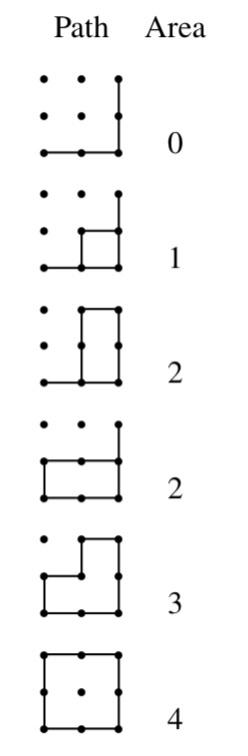
\includegraphics[scale=0.21]{latticepath.PNG}
            \caption{格路}
        \end{figure}
    \end{minipage}
\end{frame}

\begin{frame}
    %    {高斯系数的组合解释——格路}
    设$\mathscr{P}(m,n)$为从(0,0)点出发沿$x$轴或$y$轴的正方向每步走一个单位,最终走到$(m,n)$点的格路组成的集合.

    对$p \in \mathscr{P}(m,n)$,设$A(p)$为由格路$p$、$x$轴和直线 $x=m$包围图形的面积.
    \begin{thm}
        $$\sum_{p \in \mathscr{P}(k,n-k)} q^{A(p)} = {n\brack k}.$$
    \end{thm}
    \pause
    \pf
    我们记等式左边为$F(n,k)$,显然$F(n,0)=F(n,n)=0$.

    现考虑$p \in \mathscr{P}(k,n-k)$的两种情况:
    \begin{itemize}
        \item 如果路径$p$的最后一步是向北的,那么它是一条从 $(0,0)$ 到 $(k, n-k-1)$再接着往北一步的路径,且最后一步不会改变面积.

        \item 如果路径$p$的最后一步是向东的,那么它是一条从$(0,0)$到$(k-1, n-k)$再接着往东一步的路径,这里最后一步会使面积增加$n-k$.
    \end{itemize}

    故我们有
    $
    F(n,k)=F(n-1,k)+q^{n-k} F(n,k-1)
    $.

    再由定理\ref{qrec}知, $ {n\brack k}$也具有相同的初值条件和递推关系,因此定理得证.
\end{frame}







\begin{frame}{高斯系数的组合解释3 --- 有限域上的线性空间}
先给出有限域上的线性空间的一些概念.

设 $\mathbb{F}_q$ 为\blue{有限域}, 其中 $q=p^{r}$, $p$ 为素数.

对正整数$n$, 我们定义$V_{n}(q)$ 为$\mathbb{F}_q$ 上的有序 $n$ 元组
\begin{align*}
    \left(x_{1}, x_{2}, \ldots, x_{n}\right), \quad x_{i} \in \mathbb{F}_q, \quad i=1,2, \cdots, n
\end{align*}
组成的集合,并满足线性运算
\begin{align*}
    \begin{array}{c}
        \left(x_{1}, x_{2}, \cdots, x_{n}\right)+\left(y_{1}, y_{2}, \cdots, y_{n}\right)=\left(x_{1}+y_{1}, x_{2}+y_{2}, \cdots, x_{n}+y_{n}\right) \\
        \alpha\left(x_{1}, x_{2}, \cdots, x_{n}\right)=\left(\alpha x_{1}, \alpha x_{2}, \cdots, \alpha x_{n}\right), \quad \alpha \in \mathbb{F}_q
    \end{array}
\end{align*}
则 $V_n(q)$ 构成 $\mathbb{F}_q$ 上的 \blue{$n$维线性空间}, 其中的元素称为\blue{向量}.

若向量 $X_{1}, X_{2}, \cdots, X_{m}$ 满足
\begin{align*}
    \sum_{i=1}^{m} \alpha_{i} X_{i}=0, \, \alpha_{i} \in \mathbb{F}_q \Rightarrow \alpha_{i}=0, \quad i=1,2, \cdots, m
\end{align*}
则称向量 $X_{1}, X_{2}, \cdots, X_{m}$ 是\blue{线性无关}的.

\end{frame}


\begin{frame}
线性空间$V_n(q)$ 中线性无关的向量组$X_{1}, X_{2}, \cdots, X_{n}$构成 $V_n(q)$ 的一组\blue{基}.


$V_n(q)$中的任意向量都可以由 $V_n(q)$ 的一组基线性表示,
 即 对任意向量$ X \in V_n(q)$, 存在$\mathbb{F}_q$上的一组数$\alpha_{1}, \alpha_{2}, \cdots, \alpha_{n}$, 使得
\begin{align*}
    X=\sum_{i=1}^{n} \alpha_{i} X_{i}.
\end{align*}


用坐标表示为
\begin{align*}
    X=\left(\alpha_{1}, \alpha_{2}, \ldots, \alpha_{n}\right) .
\end{align*}

高斯系数${n\brack
    k}$的组合含义由下面定理给出.


\begin{thm}
    有限域 $\mathbb{F}_q$ 上的$n$维线性空间$V_n(q)$的所有$k$维子空间的个数是${n\brack k}$.
\end{thm}

例如,
 $n=3$, $k=1$时,  有限域 $\mathbb{F}_q$ 上的$3$维线性空间的所有$1$维子空间的个数是$$\frac{q^3-1}{q-1} = q^2+q+1.$$

\end{frame}


\begin{frame}
\begin{block}{定理}
    有限域 $\mathbb{F}_q$ 上的$n$维线性空间$V_n(q)$的所有$k$维子空间的个数是${n\brack k}$.
\end{block}
证明思路:
\begin{itemize}
    \item 从$V_n(q)$中选取一个由$k$个向量组成的线性无关的(有序)向量组的个数,它们生成一个$k$维子空间.
    \item 再计算一个$k$ 维子空间的(有序)基的个数.
\end{itemize}


\pf
首先,从$V_n(q)$中选取一个由$k$个向量组成的元组构成一个$k$维子空间的(有序)基.

为此,我们需要从空间$V_n(q)$中选取$k$个线性无关的向量.
\begin{itemize}
    \item 第一个向量$v_1$,可以选取任意非零向量,
    因此由$q^n-1$中选择.

    \item 第二个向量$v_2$,不能选取$v_1$的倍数,因此有$q^n-q$种选择.

    \item 第三个向量$v_3$,有$q^2$ 个不能选取的向量,它们是$v_1$和$v_2$的线性组合.
\end{itemize}



以此类推,从$V_n(q)$中选取$k$ 个线性无关的向量的方法数为
\begin{equation}\label{v_n(q)}
    (q^n-1)(q^n-q)\cdots(q^n-q^{k-1}),
\end{equation}
\end{frame}


\begin{frame}
\begin{block}{定理}
有限域 $\mathbb{F}_q$ 上的$n$维线性空间$V_n(q)$的所有$k$维子空间的个数是${n\brack k}$.
\end{block}


\indent 其次,一个子空间可以有很多组(有序)基.


类似上面的讨论,选定一个$k$ 维子空间,在其中选一组基的方法数为
		$$(q^k-1)(q^k-q)\cdots(q^k-q^{k-1}).$$
		这就是\eqref{v_n(q)}中每个子空间重复计数的数目.


        因此,$V_n(q)$的$k$维子空间的个数是
		$$\frac{(q^n-1)(q^n-q)\cdots(q^n-q^{k-1})}{(q^k-1)(q^k-q)\cdots(q^k-q^{k-1})}={n\brack k}.$$


\end{frame}

\end{document}







